\section{System Description}
The project includes many parts that must be combined to make the kart actually drive. A short description of each given part is made for easy reference.

\subsection{Go-Kart Frame}
The Go-Kart itself consists of a pre assembled aluminium frame with wheels, steering column, break pedal and seat all pre attached to the frame. The kart is big enough to fit an adult in the seat.

Behind the seat a plate is attached to fit all power electronics and drive systems produced in this project.

To the right of the driver a mount is positioned for the motor, which is protected by a metal cover. There is also a gear to transfer power better to the wheels.

The kart has a pre installed break pedal attached to a disc break by a mechanical system of springs. The speeder pedal is also installed, but nothing is attached to it, so it has no function initially.

\begin{figure}[!h]
	\centering
	\begin{subfigure}[t]{.35\linewidth}
		\includegraphics[width=\textwidth]{graphics/Gokart_Frame}
		\caption{Picture of the go kart frame}
		\label{fig:Kart_picture1}
	\end{subfigure}
	\hspace{2cm}
	\begin{subfigure}[t]{.35\linewidth}
		\includegraphics[width=\textwidth]{graphics/me1117_1}
		\caption{Picture of the Me1117 PMAC motor}
		\label{fig:The Me1117 PMAC}
	\end{subfigure}		
	\caption{Picture of the go kart and the PMAC motorl}
	\label{fig:Motor_picture1}
\end{figure}
\todo{better pic of motor}

\subsection{Battery Supply}
The batteries provided for this project are called: "SB12V20P-FC Super B
Lightweight Lithium Ion starter battery". \todo{cite datasheet}
Four of these batteries will be combined in a single supply package yielding a combined nominal voltage of 52.8V and a discharge current of 560A. The discharge current can go up to as much as 1200A for a single second of pulse.
The batteries are relatively  small at $\approx 238x120x82mm$ and $3.2kg$ of weight each.
This battery pack will be providing all the required power for the go-kart, including the motor and all control and drive circuits.


\subsection{PMAC Motor}
The PMAC motor provided is a three phase motor capable of 



\subsection{Torque Pedal}
The torque pedal or "speeder" is provided as well. It consists of a levered variable resistor with the equivalent diagram seen on figure \ref{fig:Torque_pedal_diagram}.

The torque pedal will be used to control the speed by increasing or lowering the resistance, resulting in a change of voltage on the return wires. Measuring the pedal, it is found to have a variable resistance of 0k to 7.5k. It is also found to be inaccurate in the decimals while holding a position, meaning some kind of filter might be necessary.

\begin{figure}[!h]
	\centering
	\begin{subfigure}[t]{.35\linewidth}
			\includegraphics[width=\textwidth]{graphics/torque_pedal_diagram}
			\caption{Diagram of the torque pedal}
			\label{fig:Torque_pedal_diagram}
	\end{subfigure}
	\hspace{2cm}
	\begin{subfigure}[t]{.35\linewidth}
		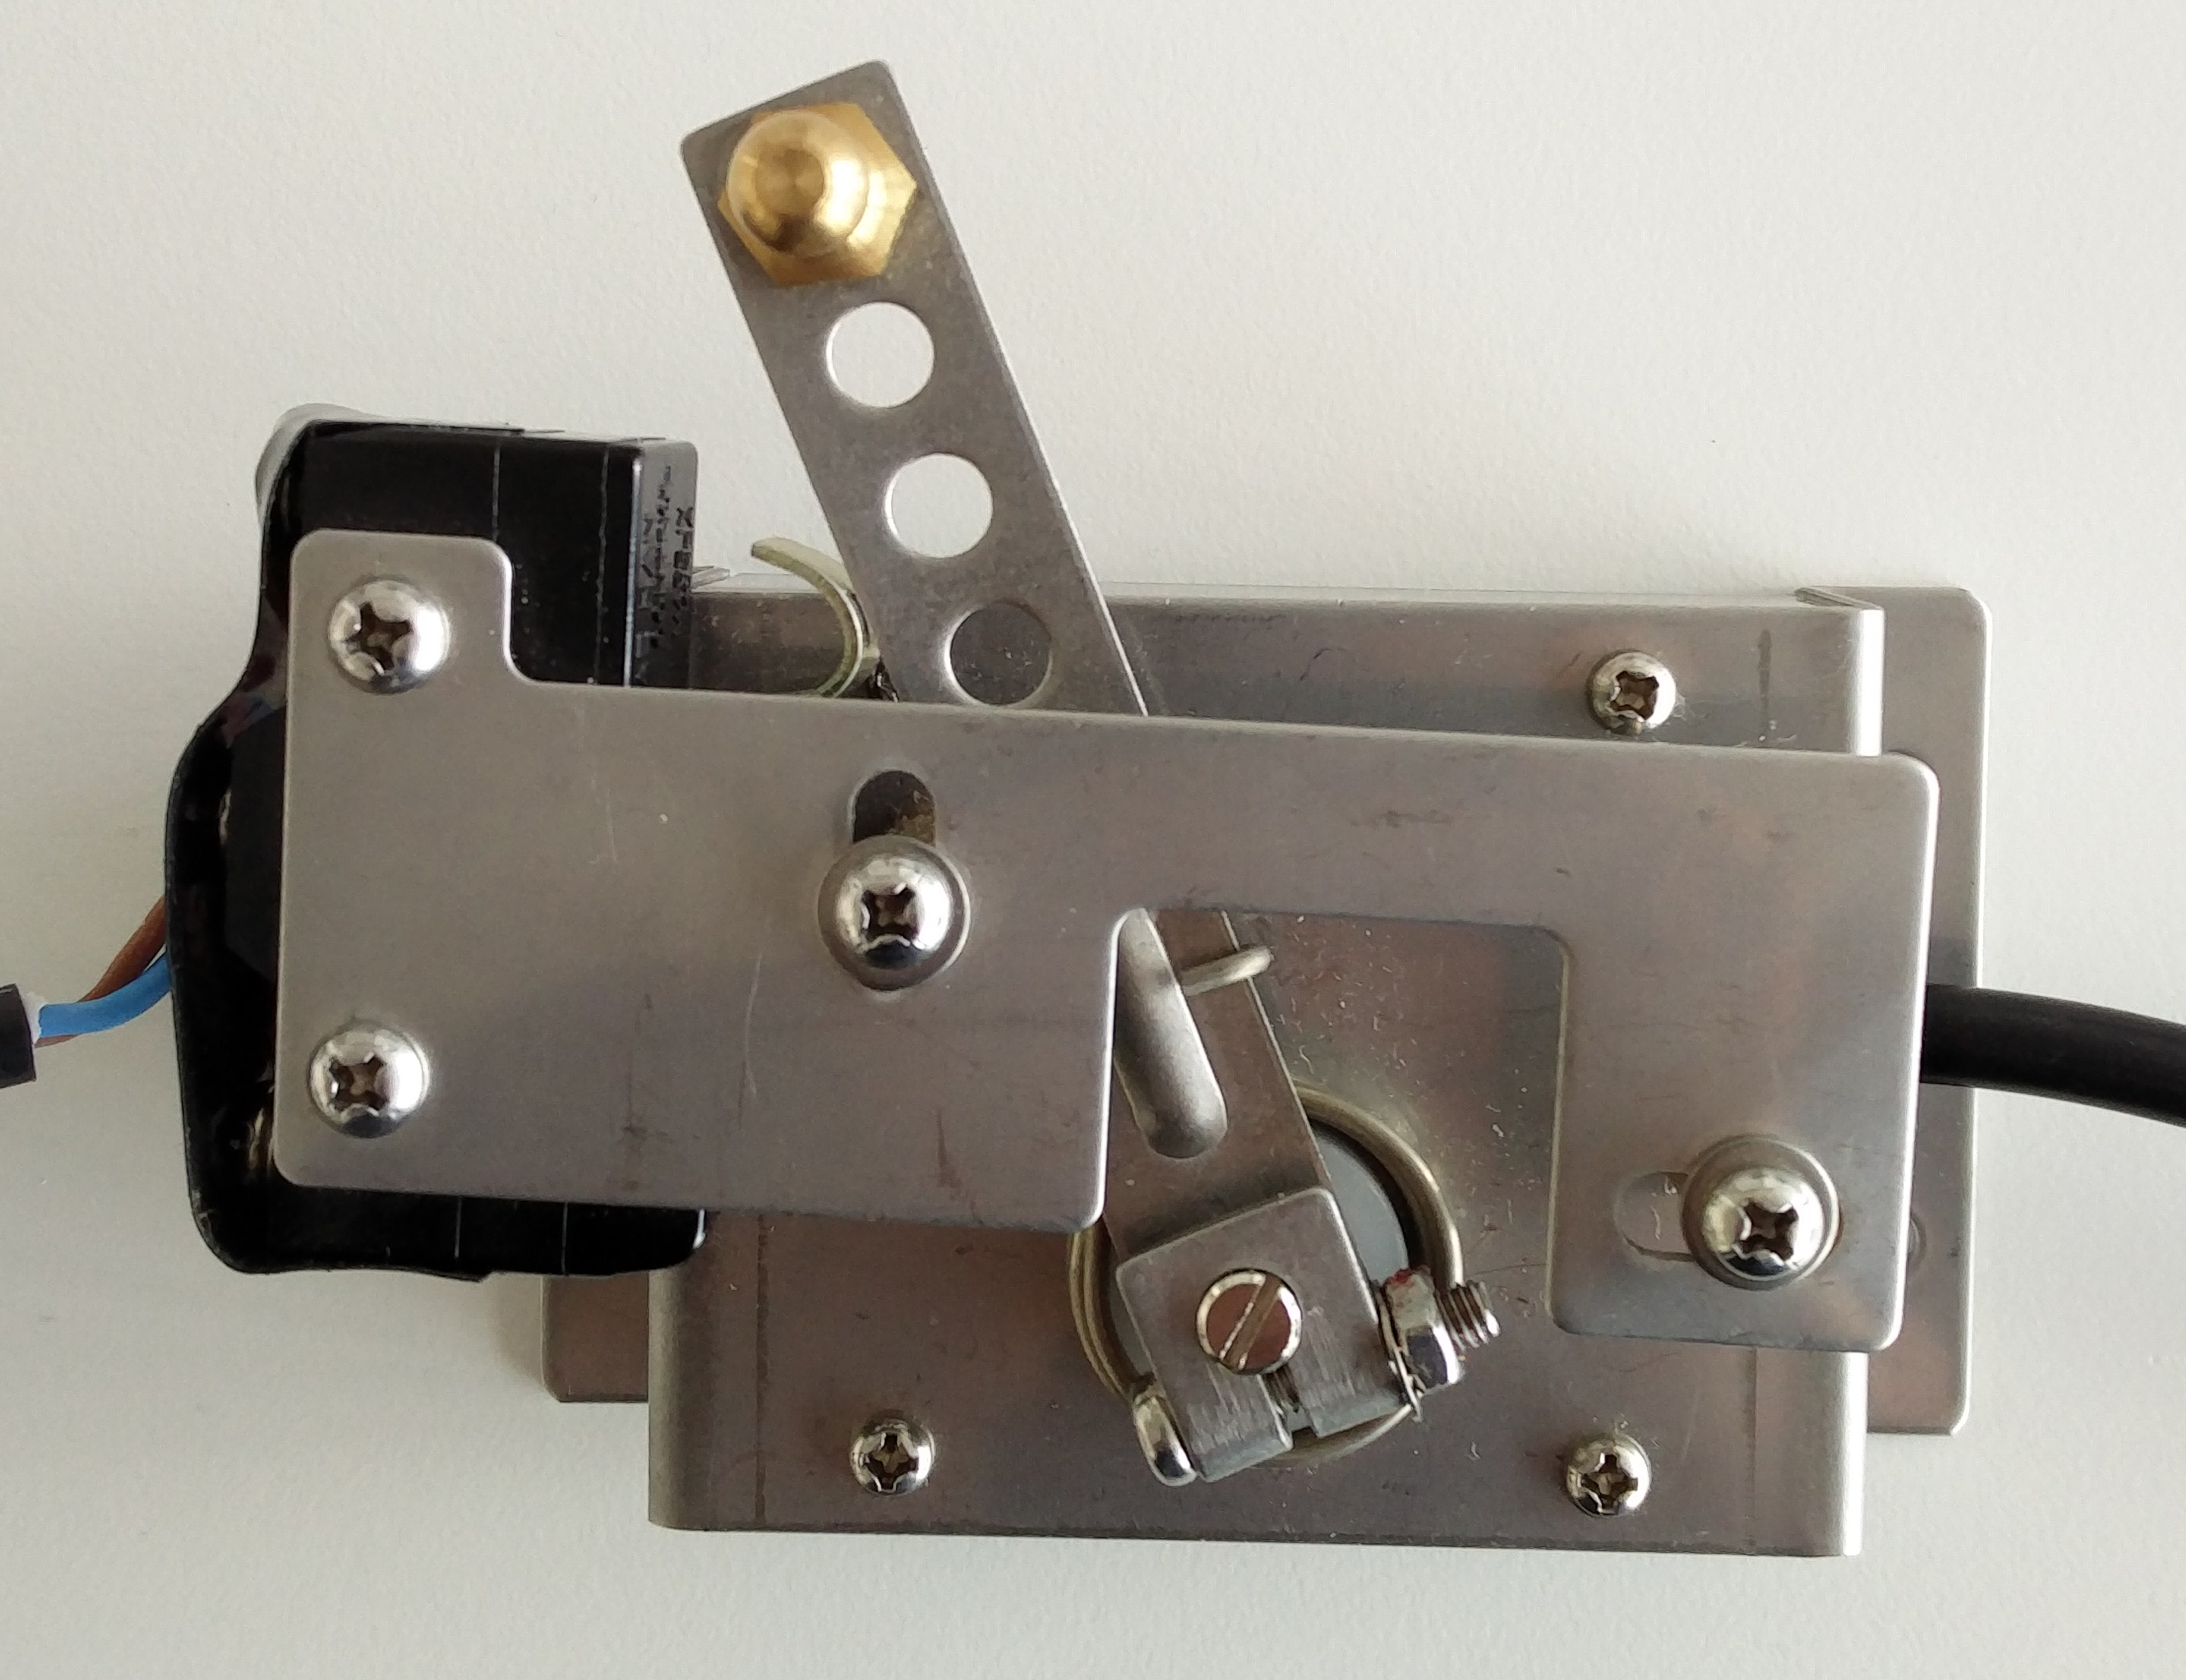
\includegraphics[width=\textwidth]{graphics/torque_pedal_picture}
		\caption{Picture of the actual torque pedal}
		\label{fig:Torque_pedal_picture}
	\end{subfigure}
	\caption{Diagram and picture of the torque pedal}
	\label{fig:Torque_pedal_diagram}
\end{figure}

\subsection{Switches and Wireing}
The wiring of the kart frame is not pre-assembled, but has been provided by the supervisors of the project, as this is standardized across multiple projects. A diagram of the wiring can be seen on figure \ref{fig:Kart_wiring_diagram}.\newline

The diagram shows the Sevcon Gen4 controller as the centrepiece surrounded by the other active parts. The motor to the right. The torque pedal, battery, undervoltage protection and multiple switches to the left. The switches include a key switch to turn the system on, an emergency switch, and a drive enable switch to change between forward or backwards drive.

\begin{figure}[!h]
	\centering
	\includegraphics[width=.95\linewidth]{graphics/Electrical_wiring_diagram_ver3}
	\caption{Diagram of go kart wiring}
	\label{fig:Kart_wiring_diagram}
\end{figure}



\clearpage